\section{Resultados}

Os programas foram compilados e executados de modo automatizado por \emph{shell scripts} no computador de um dos integrantes do grupo do trabalho. Seguem as especificações desse computador:

\begin{verbatim}Phoronix Test Suite v5.2.1
System Information

Hardware:
Processor: Intel Core i7-3612QM @ 3.10GHz (8 Cores),
Motherboard: Dell 0DNMM8, Chipset: Intel 3rd Gen Core DRAM, Memory: 8192MB,
Graphics: Intel HD 4000 2048MB (1100MHz)

Software:
OS: Fedora 20, Kernel: 3.15.10-201.fc20.x86_64 (x86_64),
Compiler: GCC 4.8.3 20140624, File-System: ext4
\end{verbatim}

\subsection{Gauss-Legendre \emph{vs} Borwein (1984)}

A especificação do trabalho pede para que os programas retornem o número $\pi$ com precisão $d = 6$ casas corretas considerando um quantidade de iterações $N = 10^9$. Porém, para os algoritmos de Gauss-Legendre e Borwein (1984), essa precisão do $\pi$ é alcançada rapidamente com a apenas $N = 2$ iterações. Diante disso, com o objetivo de ``estressar" as implementações desses algoritmos, foram criados casos de testes para alcançar precisão $d = 10^i, i = 4, 5, 6, 7$.

Para conferir a corretude dos dígitos calculados, eles foram comparados com os dígitos gerados pelo programa \texttt{pi} da CLN\cite{programa-pi} da seguinte maneira: executou-se \texttt{pi} para as precisões $d = 10^i, i = 4, 5, 6, 7$ redirecionando a saída para arquivos nomeados de acordo com $d$, e então gerou-se uma lista \texttt{md5sum} desses arquivos à qual as saídas deste trabalho foram comparadas.

\begin{table}[h]
\begin{center}
	\begin{tabular}{ |c||c|c|c||c|c|c| } 
		\hline
		Precisão & GL & GLP &  \textit{Speedup} GL & B & BP & \textit{Speedup} B \\
		\hline

		$10^4$ & 0.05   & 0.03   & 1.66 & 0.09   & 0.09   & 1.00 \\
		$10^5$ & 0.89   & 0.82   & 1.09 & 2.26   & 2.38   & 0.95 \\
		$10^6$ & 21.53  & 20.79  & 1.04 & 54.36  & 48.58  & 1.12 \\
		$10^7$ & 365.77 & 330.42 & 1.1  & 938.84 & 765.62 & 1.23 \\
		
		\hline
	\end{tabular}
	\caption{Tempos (s) de execução e \emph{speed-up} dos algoritmos Gauss-Legendre e Borwein (1984)}
	\caption*{
		GL:  Gauss-Legendre Sequencial / GLP: Gauss-Legendre Paralelo\\
		B:   Borwein (1984) Sequencial / BP:  Borwein (1984) Paralelo
	}
\end{center}
\end{table}

\begin{figure}[h]
\centering
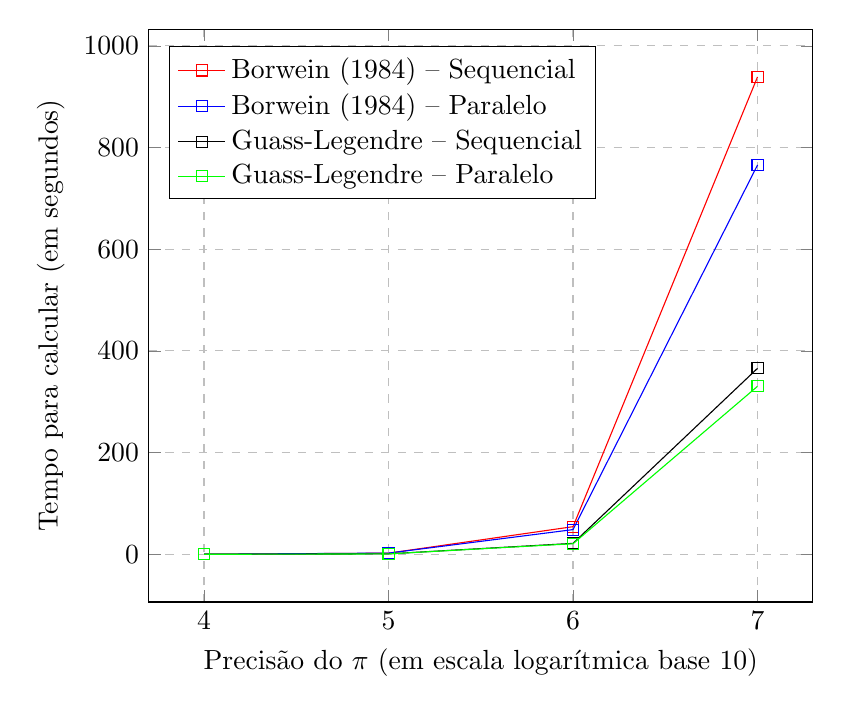
\begin{tikzpicture}
\begin{axis}[
	ylabel={Tempo para calcular (em segundos)},
	xlabel={Precisão do $\pi$ (em escala logarítmica base $10$)},
	legend cell align=left,
	legend pos=north west,
	ymajorgrids=true,
	xmajorgrids=true,
	grid style=dashed,
	/pgf/number format/1000 sep={},
	scale only axis,
	xtick = {4,5,6,7}
]
\addplot[color=red,mark=square]
coordinates{
	(4, 0.09)
	(5, 2.26)
	(6, 54.36)
	(7, 938.84)
};
\addlegendentry{Borwein (1984) -- Sequencial}

\addplot[color=blue,mark=square]
coordinates{
	(4, 0.09)
	(5, 2.38)
	(6, 48.58)
	(7, 765.62)
};
\addlegendentry{Borwein (1984) -- Paralelo}

\addplot[color=black,mark=square]
coordinates{
	(4, 0.05)
	(5, 0.89)
	(6, 21.53)
	(7, 365.77)
};
\addlegendentry{Guass-Legendre -- Sequencial}

\addplot[color=green,mark=square]
coordinates{
	(4, 0.03)
	(5, 0.82)
	(6, 20.79)
	(7, 330.42)
};
\addlegendentry{Guass-Legendre -- Paralelo}

\end{axis}
\end{tikzpicture}
\caption{Comparativo dos dados do cálculo do $\pi$ com Gauss-Legendre e Borwein (1984). \label{fig:gs-b}}
\end{figure}

Como podemos observar a partir de uma análise do \emph{speedup} de cada algoritmo, a implementação paralela torna-se mais rápida conforme a precisão requerida do $\pi$ aumenta. Porém, tal ganho do programa paralelo mostra-se ser pouco significativo se considerarmos a quantidade de \textit{threads} usadas -- 5 para Gauss-Legendre e 4 para Borwein (1984).

\subsection{Método de Monte Carlo}

Os testes do Monte Carlo para cálculo do $\pi$ foram feitos com uma quantidade fixa de $N = 10^9$ iterações, mas com uma quantidade váriavel de \textit{threads} o que nos possibilitou conferir o tempo de execução do programa de acordo com a quantidade de \textit{threads} utilizada. Pelos resultados da Tabela~\ref{tab:mc_res} pode-se perceber que o tempo de execução diminuiu conforme o aumento da quantidade de \textit{threads}, porém não de maneira proporcional.

\begin{table}[h]
\begin{center}
	\begin{tabular}{ |c|c|c|c|c| } 
		\hline
		nthreads & MC & MCP & \textit{Speedup} & $\approx \pi$ \\
		\hline

		$-$ & 29.68 & -      & -    & 3.16098686 \\
		$2$ & -     & 22.31  & 1.33 & 3.14160214 \\
		$4$ & -     & 20.61  & 1.44 & 3.14156532 \\
		$8$ & -     & 15.51  & 1.92 & 3.14165089 \\
		
		\hline
	\end{tabular}
	\caption{Tempos (s) de execução e \emph{speed-up} do Método de Monte Carlo para $\pi$ \label{tab:mc_res}}
	\caption*{
		MC:  Monte Carlo Sequencial\\
		MCP: Monte Carlo Paralelo
	}
\end{center}
\end{table}

\subsection{Black-Scholes}

Análogo aos testes do Método de Monte Carlo para $\pi$, os testes para Black-Scholes também foram feitos com uma quantidade variável de \textit{threads} e com uma entrada fixa do arquivo \texttt{entrada\char`_blackscholes.txt} que informa uma quantidade $M = 10^9$ iterações. Pelos resultados da Tabela~\ref{tab:bs_res} pode-se perceber que o tempo de execução diminuiu conforme o aumento da quantidade de \textit{threads}, porém também não de maneira proporcional.

\begin{table}[h]
\begin{center}
	\begin{tabular}{ |c|c|c|c|c| } 
		\hline
		nthreads & BS & BSP & \textit{Speedup} & intconf \\
		\hline

		$-$ & 115.95 & -     & -    & [99.986946,   99.986947] \\
		$2$ & -      & 74.67 & 1.55 & [99.989184,   99.989185] \\
		$4$ & -      & 59.66 & 1.94 & [99.983979,   99.983980] \\
		$8$ & -      & 47.62 & 2.43 & [100.000951, 100.000951] \\
		
		\hline
	\end{tabular}
	\caption{Tempos (s) de execução e \emph{speed-up} do Black-Scholes \label{tab:bs_res}}
	\caption*{
		BS:  Black-Scholes Sequencial\\
		BSP: Black-Scholes Paralelo\\
		intconf: intervalo de confiança
	}
\end{center}
\end{table}
